\chapter{Phân tích Thực nghiệm và Đối sánh Baseline}
\label{ch:phantich_sosanh}

\section{Cấu hình Phần cứng và Môi trường Đo}
Theo yêu cầu kiểm chứng tái lập của rubric CO4033, mọi thí nghiệm được tách rõ hai môi trường đo:
\begin{itemize}[leftmargin=1.5em]
  \item \textbf{Hạ tầng Pipeline Cloud \& BI Serving:} AWS \texttt{ap-southeast-1} (Lambda/SQS/S3/DynamoDB), Databricks Free Edition (\texttt{Serverless}), Neon PostgreSQL (\texttt{quick\_gold\_md01} dung lượng \texttt{449 MB}), Streamlit \texttt{1.42+}.
  \item \textbf{Máy chạy Local (ML Notebooks \texttt{NB01--NB05} \& \texttt{pytest}):} [Chờ nhóm điền cấu hình máy thực tế chạy đo, ví dụ: CPU Intel/AMD ..., RAM ... GB, Windows 11, Python \texttt{3.12.10} trong \texttt{.venv}].
\end{itemize}

\section{Chẩn đoán Thống kê 8 Nhóm ATC (\texttt{NB02})}
Trên tập quan sát thực \texttt{store\_id = 5631} (\texttt{302} tuần, \texttt{2,106} ngày), phân loại Syntetos--Boylan \cite{syntetos2005} và kiểm định tương quan thời tiết ERA5 (Hình~\ref{fig:eda_quadrant} và Hình~\ref{fig:eda_ccf}) cho thấy sự phân hóa hành vi rõ rệt giữa 8 nhóm thuốc:
\begin{itemize}[leftmargin=1.5em]
  \item \textbf{Nhóm mượt theo mùa mạnh (\textit{Smooth}):} \texttt{N02BE} (Paracetamol, TB \texttt{208.63} đv/tuần, \texttt{ACF(52) = 0.53}, bùng mạnh mùa đông) và \texttt{R06} (Kháng histamin dị ứng, \texttt{ACF(52) = 0.63}).
  \item \textbf{Nhóm biến động mạnh (\textit{Erratic}):} \texttt{R03} (Hen/COPD, \texttt{CV$^2$ = 0.82}, \texttt{23.0\%} ngày = 0).
  \item \textbf{Nhóm bán thưa (\textit{Intermittent}):} \texttt{N05C} (An thần gây ngủ, \texttt{ADI = 3.12}, \texttt{67.9\%} ngày bằng 0, \texttt{36} tuần bằng 0) --- trực tiếp lý giải vì sao \texttt{MAPE} nổ \texttt{inf\%} ở bài báo cũ \cite{fourkiotis2024} và bắt buộc phải dùng \texttt{WAPE/MASE} kèm \texttt{Croston-SBA} hoặc \texttt{LightGBM Tweedie}.
\end{itemize}

\begin{figure}[H]
\centering
\begin{subfigure}[t]{0.48\textwidth}
  \centering
  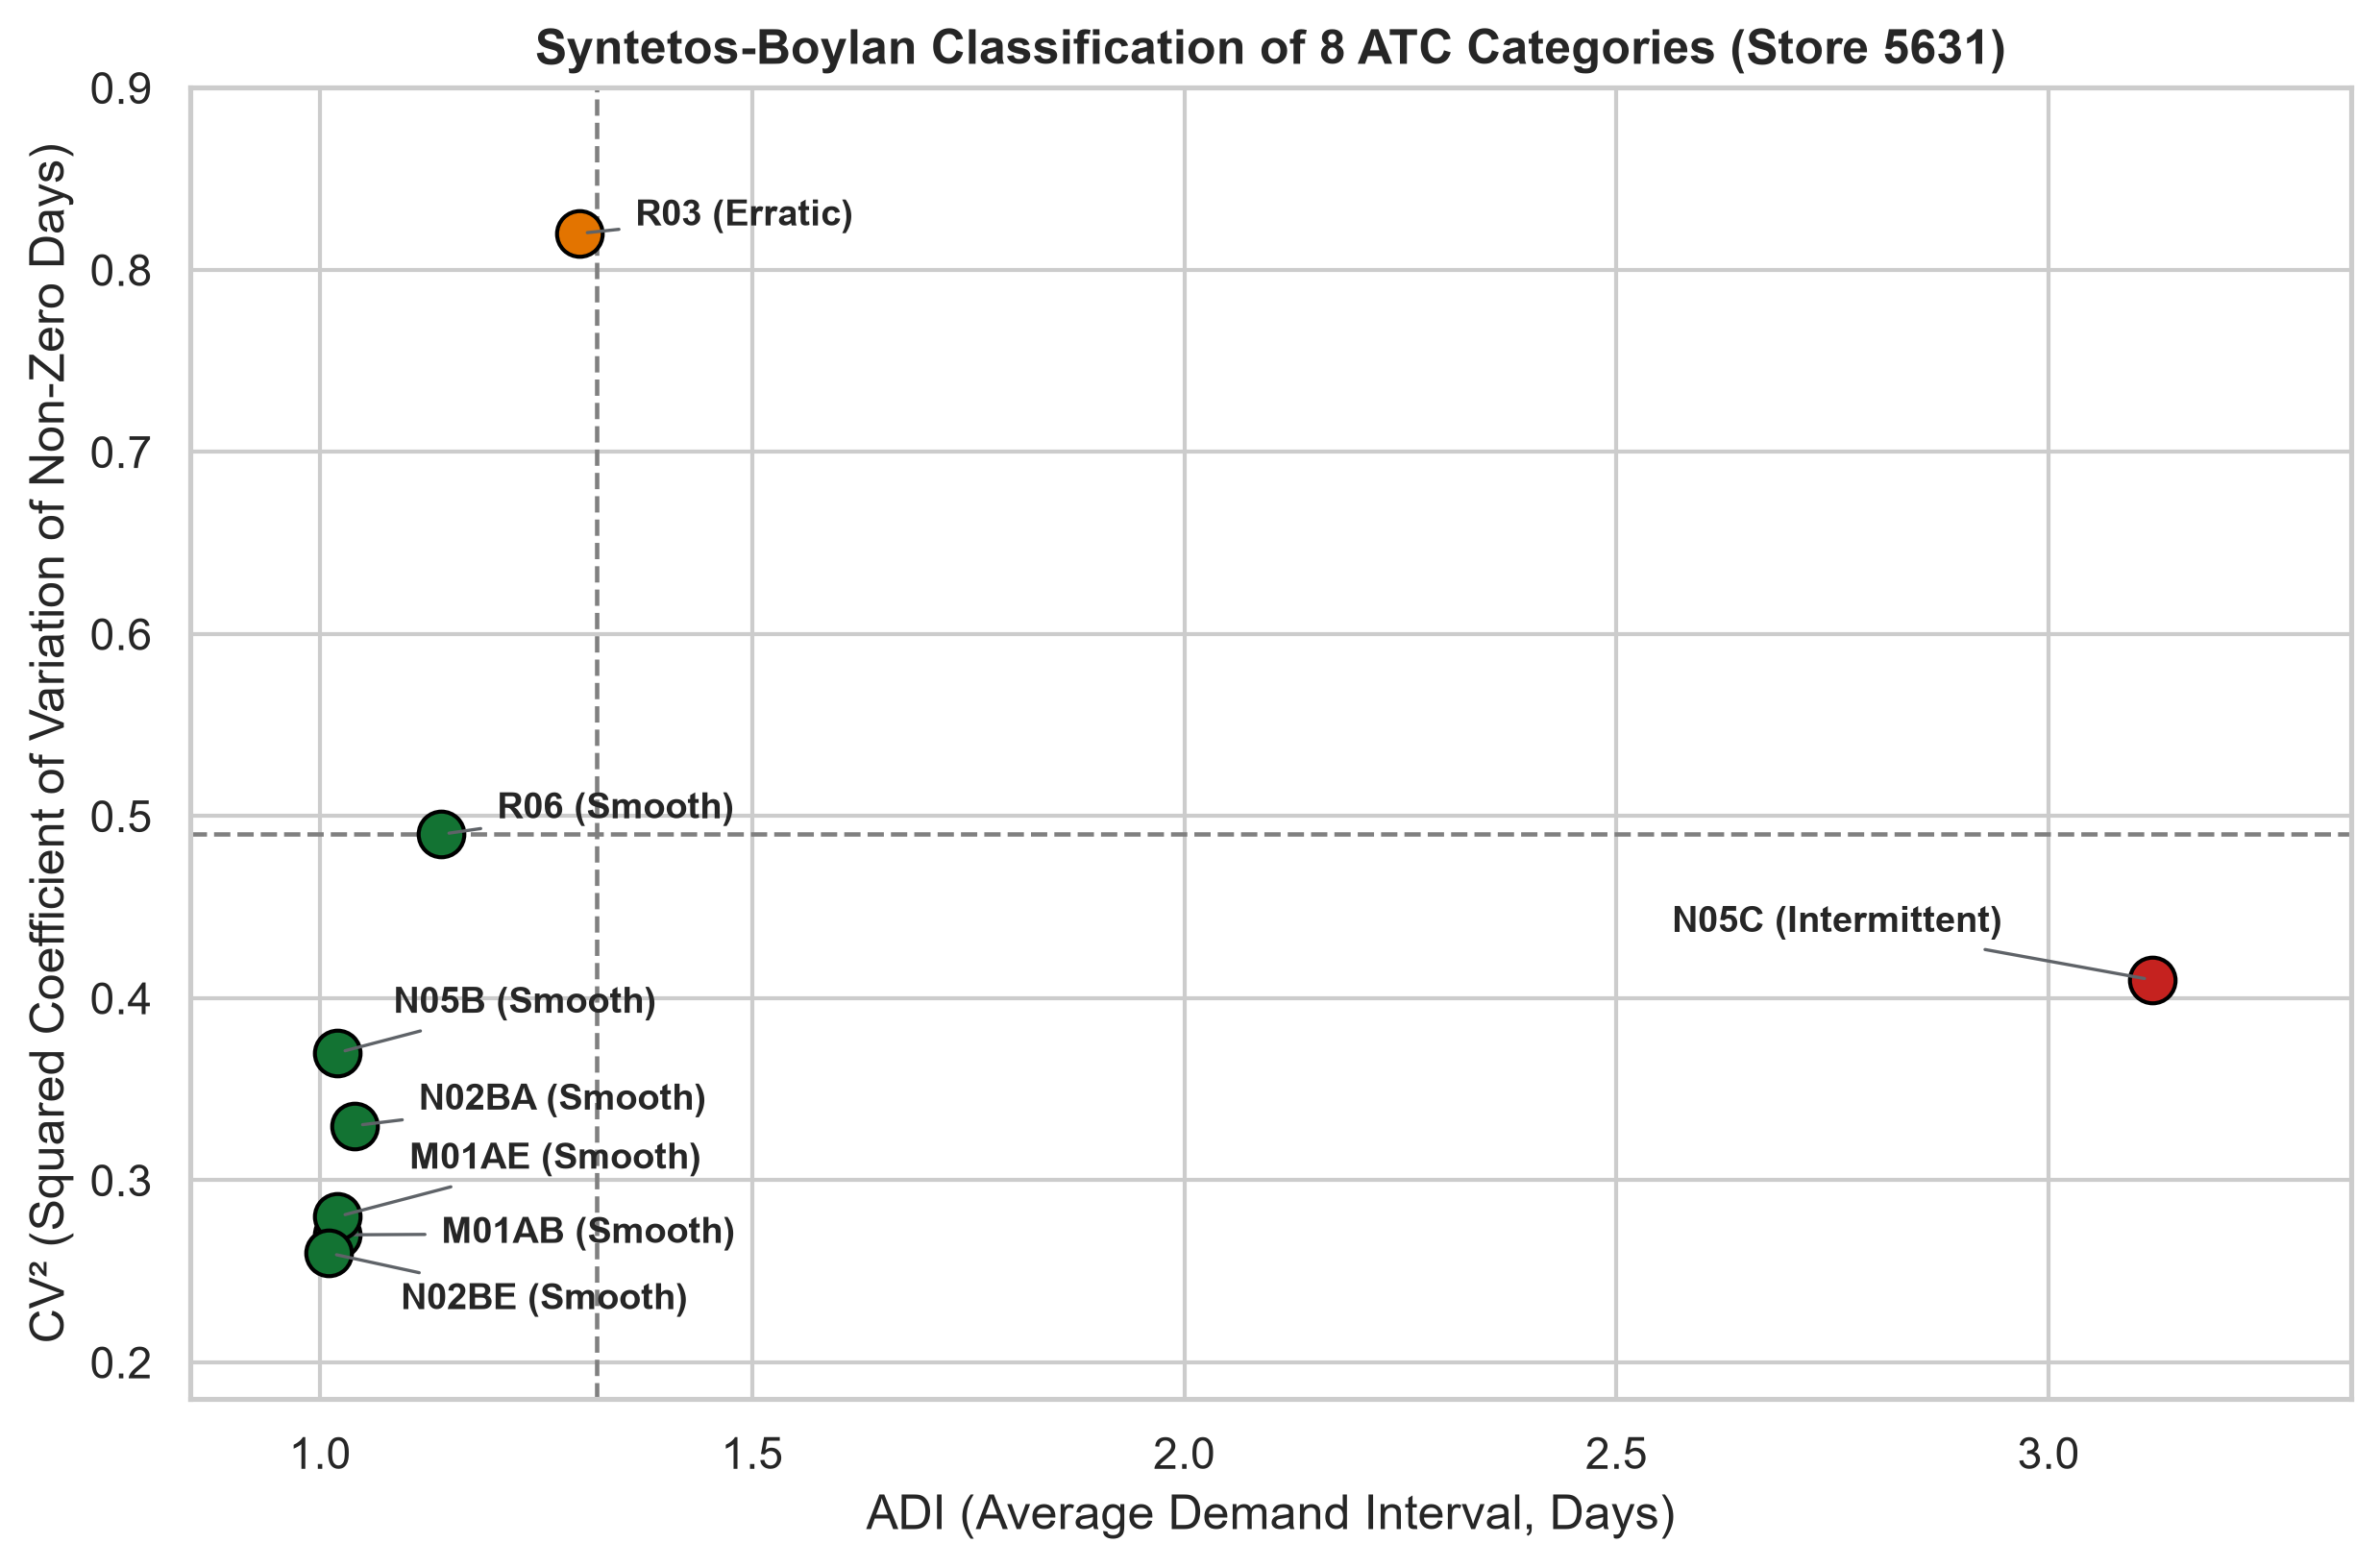
\includegraphics[width=\textwidth]{../../artifacts/forecasting/eda_02_syntetos_boylan_quadrant.png}
  \caption{Phân vùng Syntetos--Boylan (\texttt{ADI/CV$^2$})}
  \label{fig:eda_quadrant}
\end{subfigure}
\hfill
\begin{subfigure}[t]{0.48\textwidth}
  \centering
  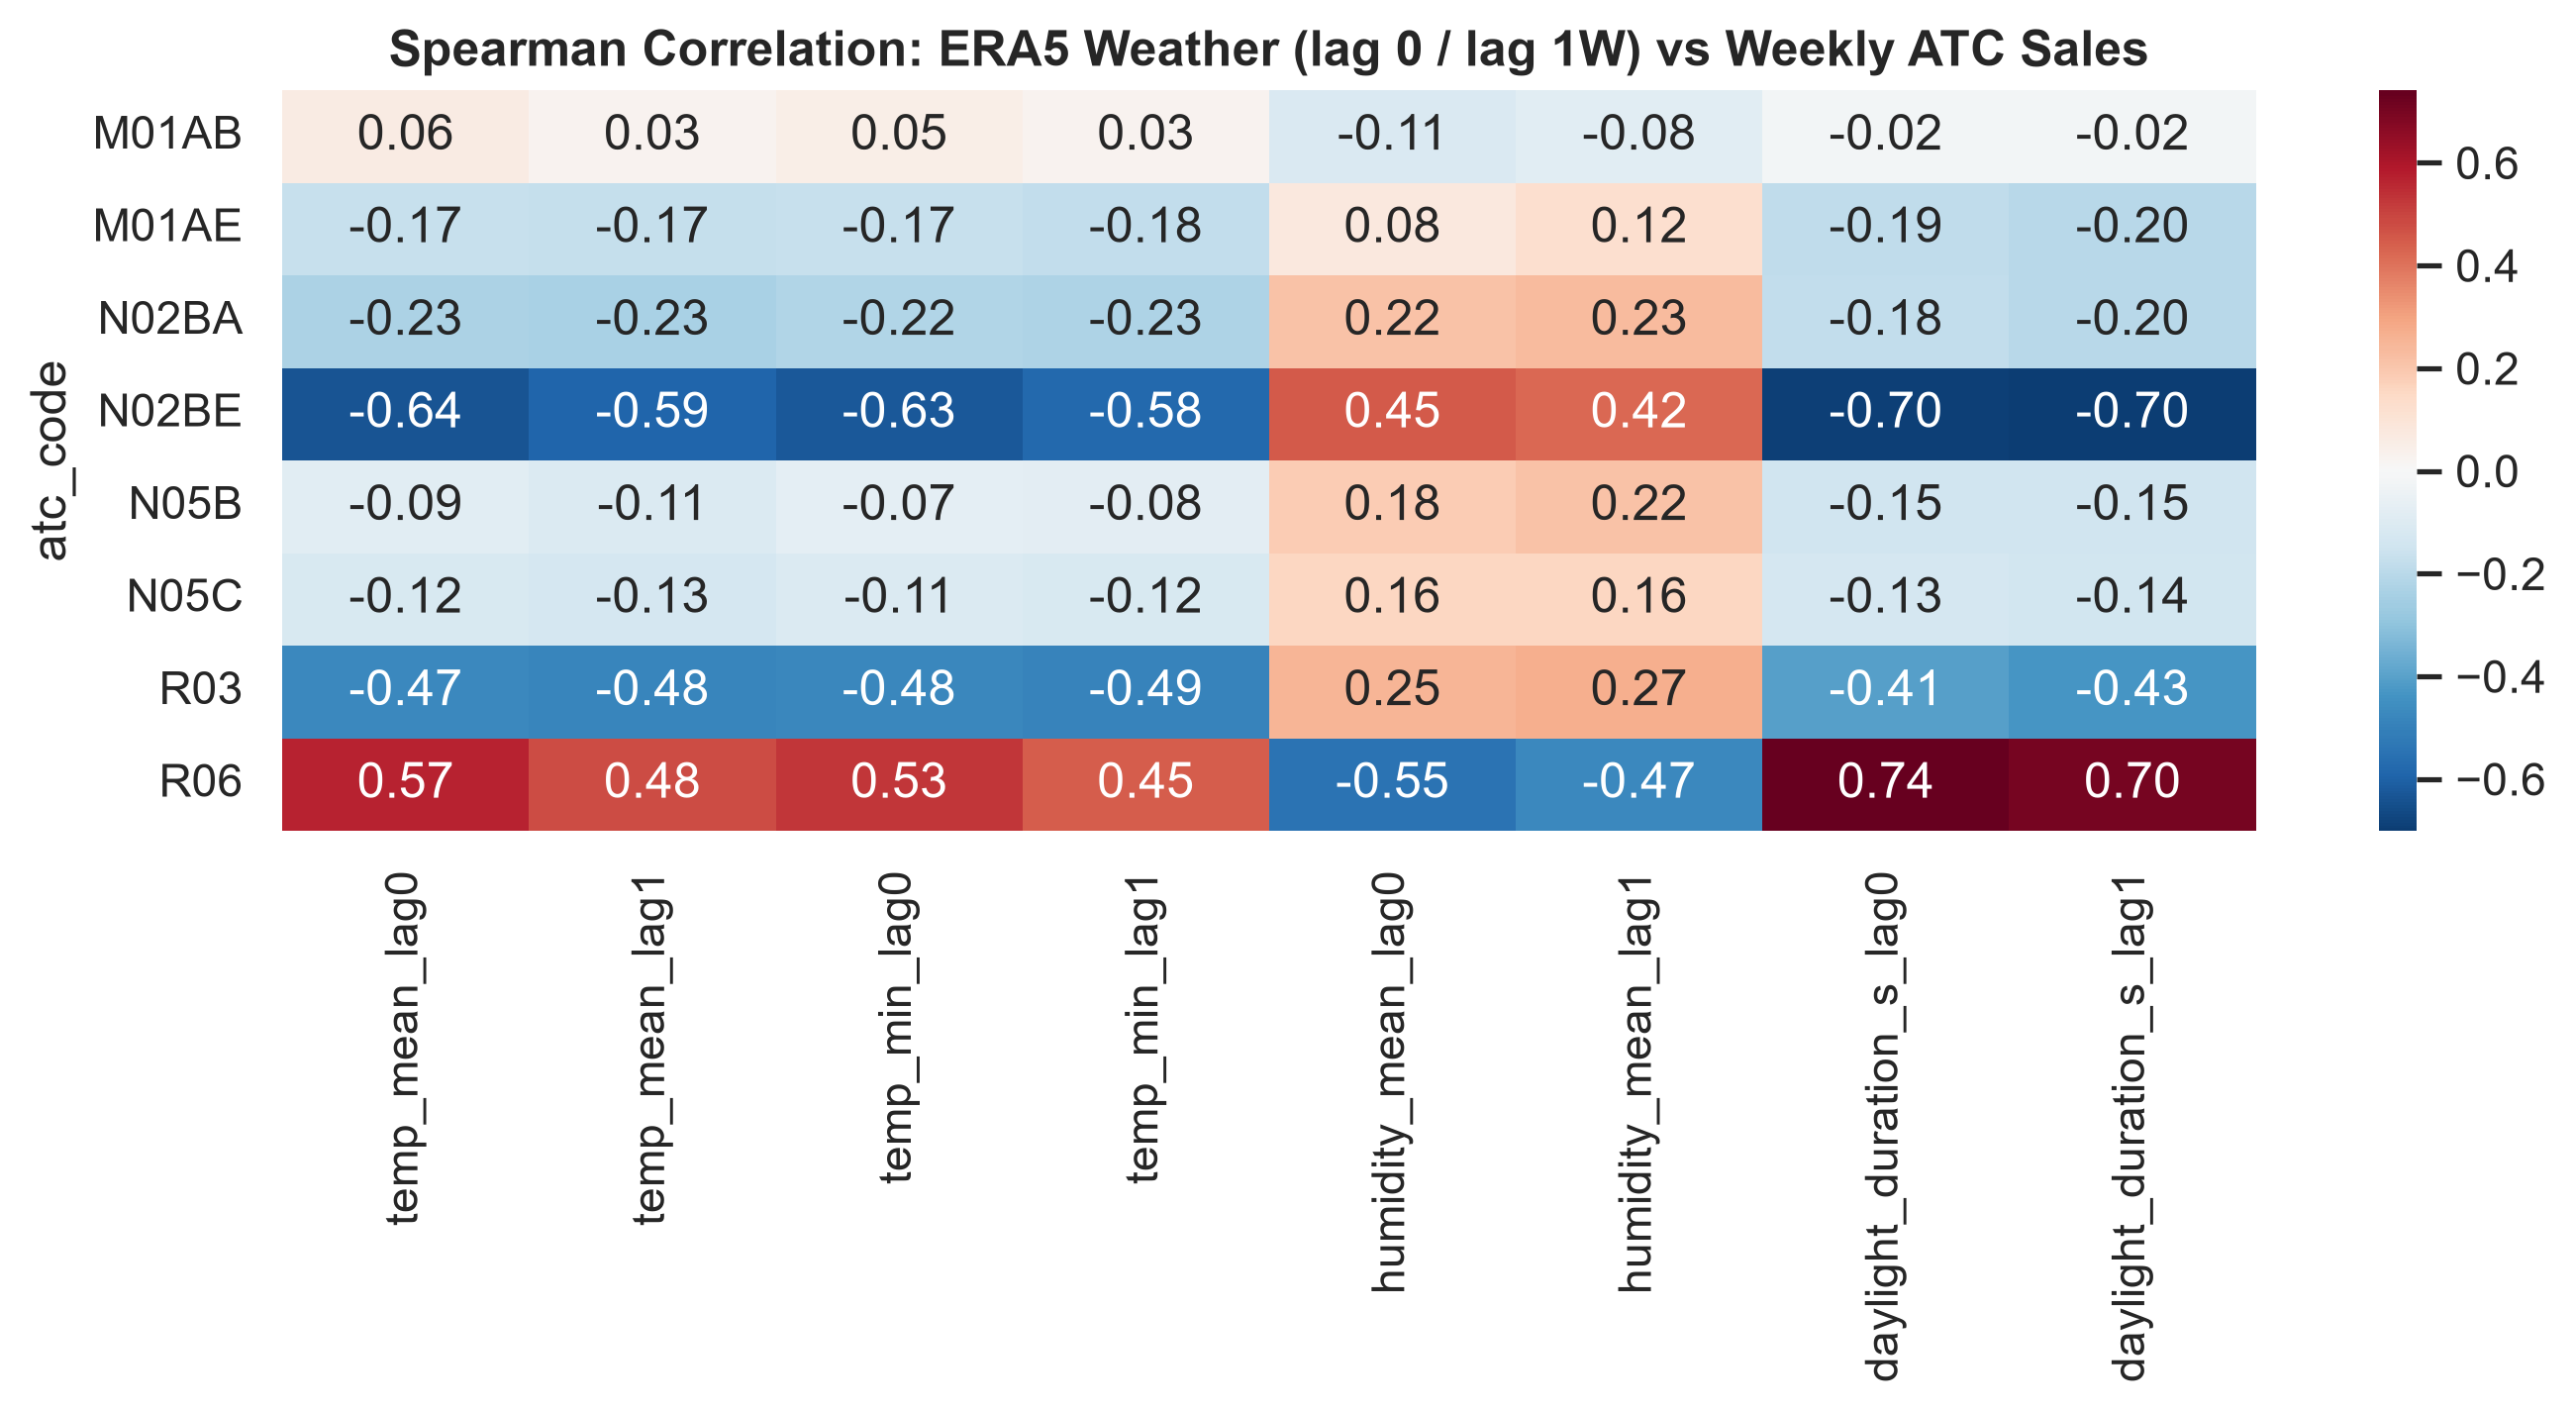
\includegraphics[width=\textwidth]{../../artifacts/forecasting/eda_04_weather_ccf.png}
  \caption{Tương quan trễ thời tiết ERA5 với doanh số}
  \label{fig:eda_ccf}
\end{subfigure}
\caption{Chẩn đoán phân loại chuỗi thời gian và tín hiệu khí tượng ERA5 trên 8 nhóm ATC}
\label{fig:eda_diag}
\end{figure}

\section{Bảng Kết quả Thực nghiệm Theo Mẫu CO4033 (Mục V)}
Bảng~\ref{tab:co4033_exp_summary} tổng hợp kết quả đo đạc thực tế giữa Baseline và Giải pháp đề xuất cho cả hai mảng chính (ML Forecasting và BI Serving).

\begin{table}[H]
\centering
\caption{Bảng tổng hợp thực nghiệm đối chiếu Baseline và Giải pháp đề xuất theo mẫu Mục V Rubric CO4033}
\label{tab:co4033_exp_summary}
\renewcommand{\arraystretch}{1.22}
\begin{tabularx}{\textwidth}{|p{0.21\textwidth}|p{0.25\textwidth}|p{0.26\textwidth}|X|}
\hline
\textbf{Chỉ số} & \textbf{Baseline} & \textbf{Giải pháp đề xuất} & \textbf{Nhận xét} \\
\hline
Số bản ghi đầu vào & \texttt{16,848} dòng ATC (2014--2019); \texttt{474,591} dòng Gold POS & Đồng bộ toàn bộ nguồn trên cộng \texttt{2,080} ngày ERA5 (\texttt{19,902} tệp JSON gốc) & Giữ nguyên \texttt{100\%} quan sát thực \texttt{OBSERVED}, không bịa thiếu hàng. \\
\hline
Tỷ lệ dữ liệu lỗi/thiếu & \texttt{uv\_index\_max} thiếu \texttt{100\%}; \texttt{26} ngày lễ khuyết ERA5; \texttt{W302} hụt \texttt{2/7} ngày & Loại \texttt{uv\_index\_max}; thuần \texttt{.ffill()}; chuẩn hóa \texttt{qty\_rate} & Perturbation Leakage Unit-Test \texttt{= 0.0}; loại bỏ cảnh báo giả ở \texttt{W302}. \\
\hline
Thời gian xử lý (s) & \texttt{54 giờ} Grid Search ở \cite{fourkiotis2024}; BI query: [Chờ đo baseline pandas kéo full \texttt{474K} dòng] & \textbf{ML luồng \texttt{NB01--05}: \texttt{166.6s}} (\texttt{2.78 phút}); \textbf{BI Pushdown: \texttt{0.08--0.48s}/query} & ML nhanh gấp \texttt{1,166.9$\times$} so với \cite{fourkiotis2024}; BI không tải 474K dòng về RAM. \\
\hline
Chất lượng mô hình / KPI & \texttt{SNaïve} (MSE): \texttt{N02BE 3605.15}, \texttt{N05B 450.79}, \texttt{N05C 21.75} & \texttt{AutoRouter} thắng \texttt{SNaïve} ở \textbf{\texttt{8/8} ATC} (\texttt{DM' p<0.05}); \textbf{\texttt{6/8} vượt XGB \cite{fourkiotis2024}}; CQR phủ \textbf{\texttt{78.8\%}} & Cải thiện rõ rệt trên cả \texttt{52W}, \texttt{4 Rolling Folds} và \texttt{365D}. \\
\hline
Dung lượng lưu trữ (MB) & Dữ liệu gốc tách rời 3 nguồn & Neon BI Mirror \texttt{449 MB}; Artifacts ML \texttt{artifacts/forecasting/} (\texttt{$<$ 6 MB}) & Gọn nhẹ, deploy trực tiếp trên Streamlit Cloud miễn phí. \\
\hline
Giá trị kinh doanh & Chi tiết rải rác, dễ hiểu nhầm \texttt{MAPE = inf\%} và đa ĐVT & Dashboard 5 trang tiếng Việt + giải thích \texttt{TreeSHAP} (\texttt{11.3--25.9\%} từ ERA5) & Hỗ trợ lập kế hoạch nhân sự/nhập hàng \textit{human-in-the-loop}. \\
\hline
\end{tabularx}
\end{table}

\section{Đối sánh Chi tiết Trên 8 Nhóm ATC và Kiểm chứng Khoa học}
Bảng~\ref{tab:ml_benchmark_8atc} trình bày đối sánh công bằng 2 tầng trên tập kiểm chứng 52 tuần cuối (\texttt{W251--W302}): (1) đối sánh nội bộ giữa \texttt{AutoRouted\_Champion} với \texttt{Seasonal\_Naive} và \texttt{Seasonal\_Naive\_Weighted}; (2) đối sánh tham chiếu 1:1 với Bảng 2 của Fourkiotis \& Tsadiras (2024) \cite{fourkiotis2024}.

\begin{table}[H]
\centering
\caption{Kết quả thực nghiệm 52 tuần cuối (\texttt{W251--W302}) trên 8 nhóm ATC và đối sánh Paper 2024 \cite{fourkiotis2024}}
\label{tab:ml_benchmark_8atc}
\renewcommand{\arraystretch}{1.20}
\setlength{\tabcolsep}{3.5pt}
\scriptsize
\begin{tabularx}{\textwidth}{|l|X|p{0.21\textwidth}|c|c|c|c|}
\hline
\textbf{ATC} & \textbf{\texttt{AutoRouted} (MSE / WAPE)} & \textbf{MSE Thấp nhất (PF)} & \textbf{\texttt{SNaïve}} & \textbf{XGB \cite{fourkiotis2024}} & \textbf{\texttt{DM'} \texttt{SNaïve}} & \textbf{CQR 80\%} \\
\hline
\textbf{M01AB} & \texttt{Croston\_SBA} (\texttt{58.24} / \texttt{15.74\%}) & \textbf{\texttt{Ridge\_F1F2F3}} (\texttt{52.68}) & \texttt{107.08} & \texttt{54.81} & \texttt{p=0.0100*} & \texttt{82.7\%} \\
\hline
\textbf{M01AE} & \texttt{Ridge\_F1F2F3} (\texttt{72.64} / \texttt{25.17\%}) & \texttt{AnchorRes\_F3} (\texttt{67.56}) & \texttt{105.88} & \textbf{\texttt{28.80}} & \texttt{p=0.0315*} & \texttt{63.5\%} \\
\hline
\textbf{N02BA} & \texttt{Harmonic\_ARIMA} (\texttt{29.06} / \texttt{20.92\%}) & \textbf{\texttt{LightGBM\_F1F2}} (\texttt{27.72}) & \texttt{52.07} & \texttt{40.69} & \texttt{p=0.0071*} & \texttt{75.0\%} \\
\hline
\textbf{N02BE} & \texttt{LightGBM\_F1F2F3} (\texttt{2042.8} / \texttt{15.44\%}) & \textbf{\texttt{AnchorRes\_F3}} (\texttt{1392.2}) & \texttt{3605.15} & \texttt{1518.56} & \texttt{p=0.0147*} & \texttt{78.8\%} \\
\hline
\textbf{N05B} & \textbf{\texttt{AnchorRes\_F3}} (\texttt{139.66} / \texttt{16.49\%}) & \textbf{\texttt{Ridge\_F1F2F3}} (\texttt{118.65}) & \texttt{450.79} & \texttt{260.52} & \texttt{p=0.0045*} & \texttt{73.1\%} \\
\hline
\textbf{N05C} & \texttt{LightGBM\_F1F2F3} (\texttt{8.66} / \texttt{47.94\%}) & \textbf{\texttt{Croston\_SBA}} (\texttt{7.76}) & \texttt{21.75} & \texttt{7.90} & \texttt{p=0.0043*} & \texttt{86.5\%} \\
\hline
\textbf{R03} & \texttt{AnchorRes\_F3} (\texttt{688.80} / \texttt{38.32\%}) & \texttt{Harmonic\_ARIMA} (\texttt{662.25}) & \texttt{1142.61} & \textbf{\texttt{350.84}} & \texttt{p=0.0175*} & \texttt{88.5\%} \\
\hline
\textbf{R06} & \textbf{\texttt{AnchorRes\_F3}} (\texttt{57.04} / \texttt{24.67\%}) & \textbf{\texttt{LightGBM\_F1F2}} (\texttt{49.75}) & \texttt{137.75} & \texttt{63.85} & \texttt{p=0.0011*} & \texttt{82.7\%} \\
\hline
\end{tabularx}
\end{table}

\begin{figure}[H]
\centering
\begin{subfigure}[t]{0.48\textwidth}
  \centering
  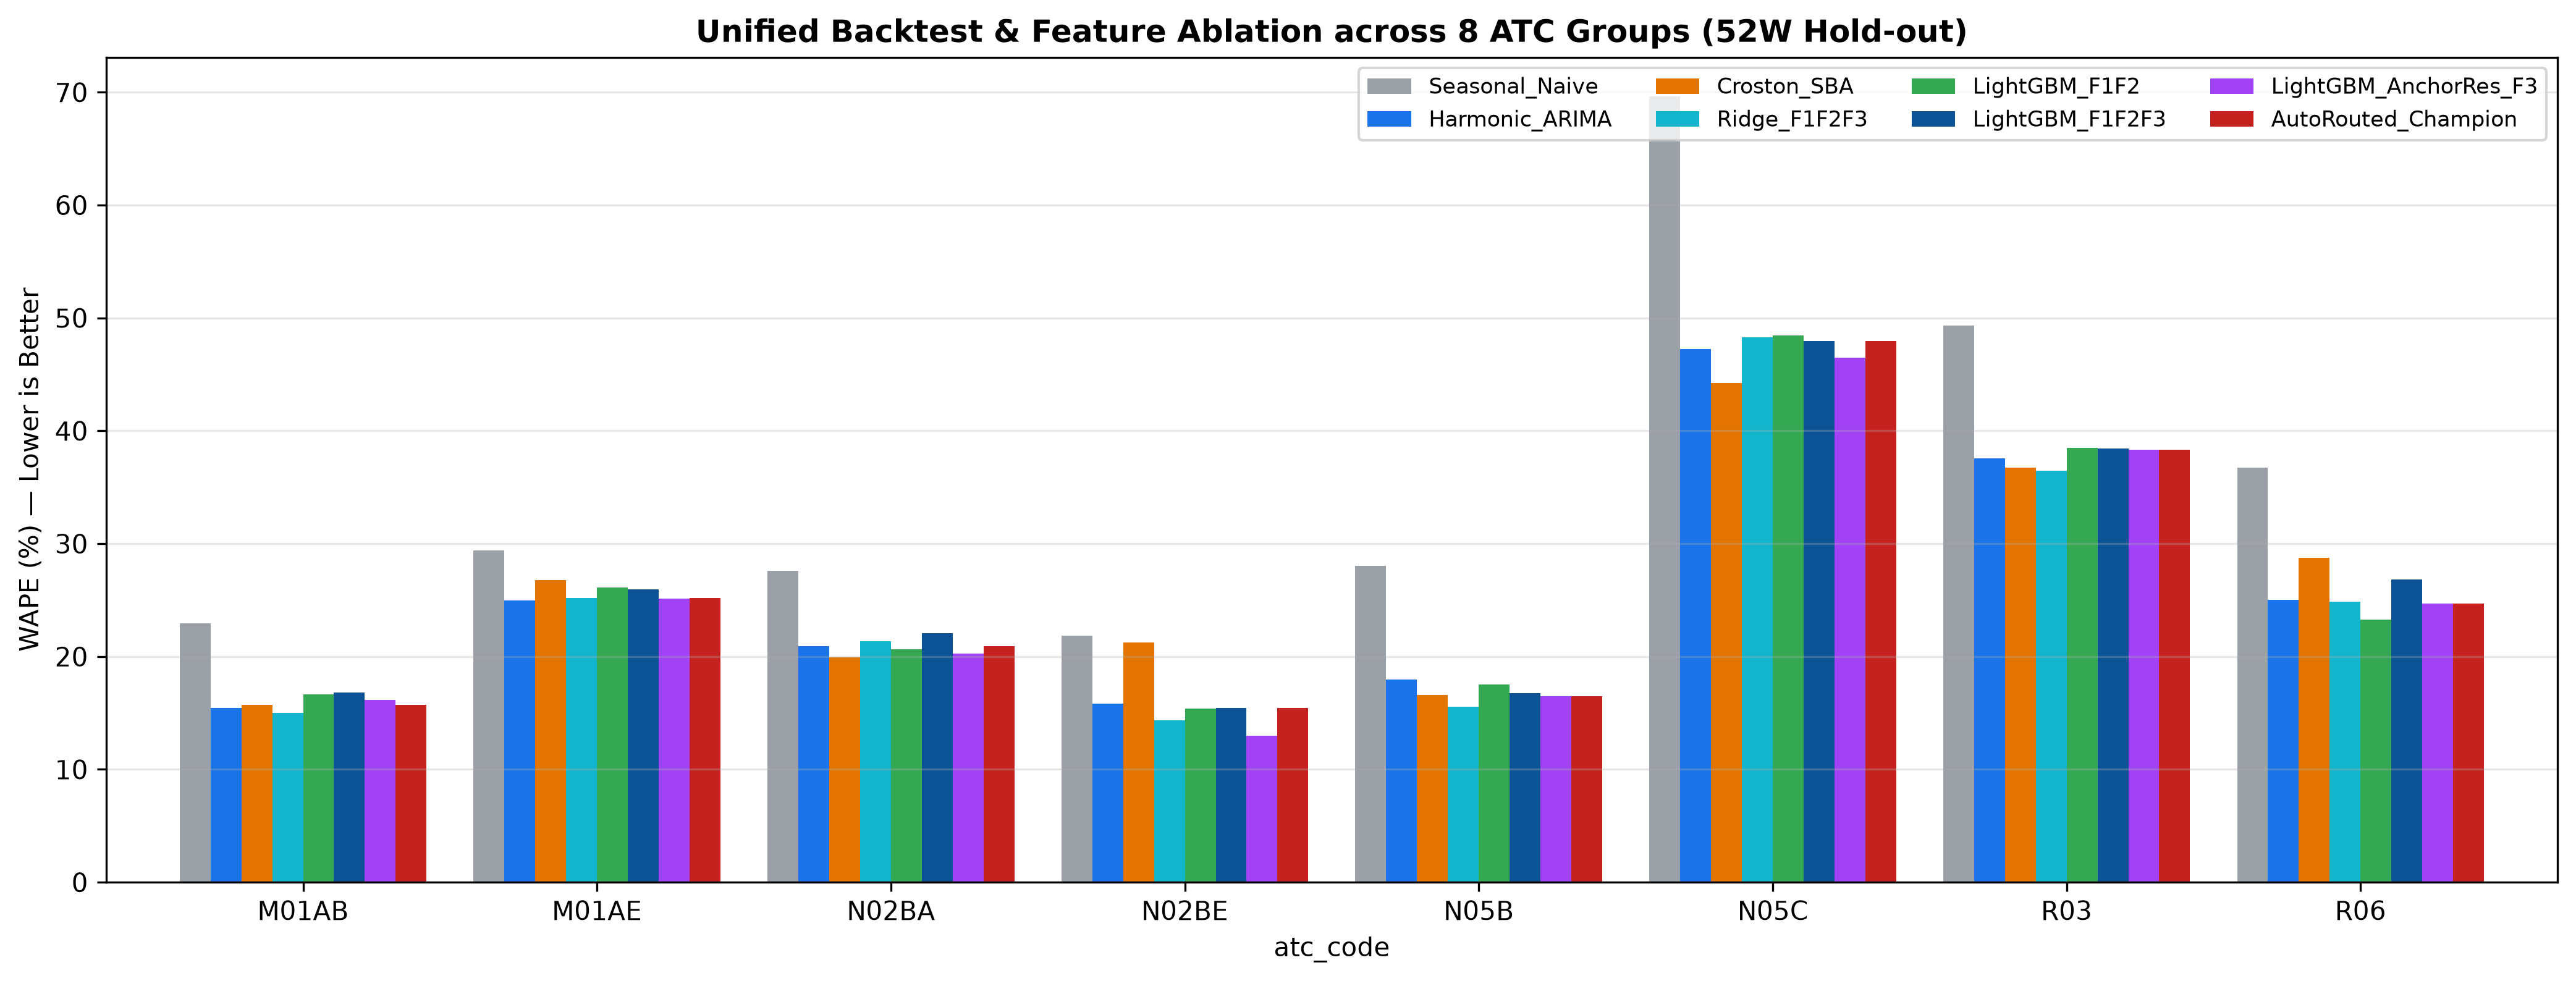
\includegraphics[width=\textwidth]{../../artifacts/forecasting/eval_ablation_wape.png}
  \caption{Ablation đặc trưng (\texttt{F1 $\rightarrow$ F1F2 $\rightarrow$ ERA5} \& \texttt{AnchorRes})}
  \label{fig:eval_ablation}
\end{subfigure}
\hfill
\begin{subfigure}[t]{0.48\textwidth}
  \centering
  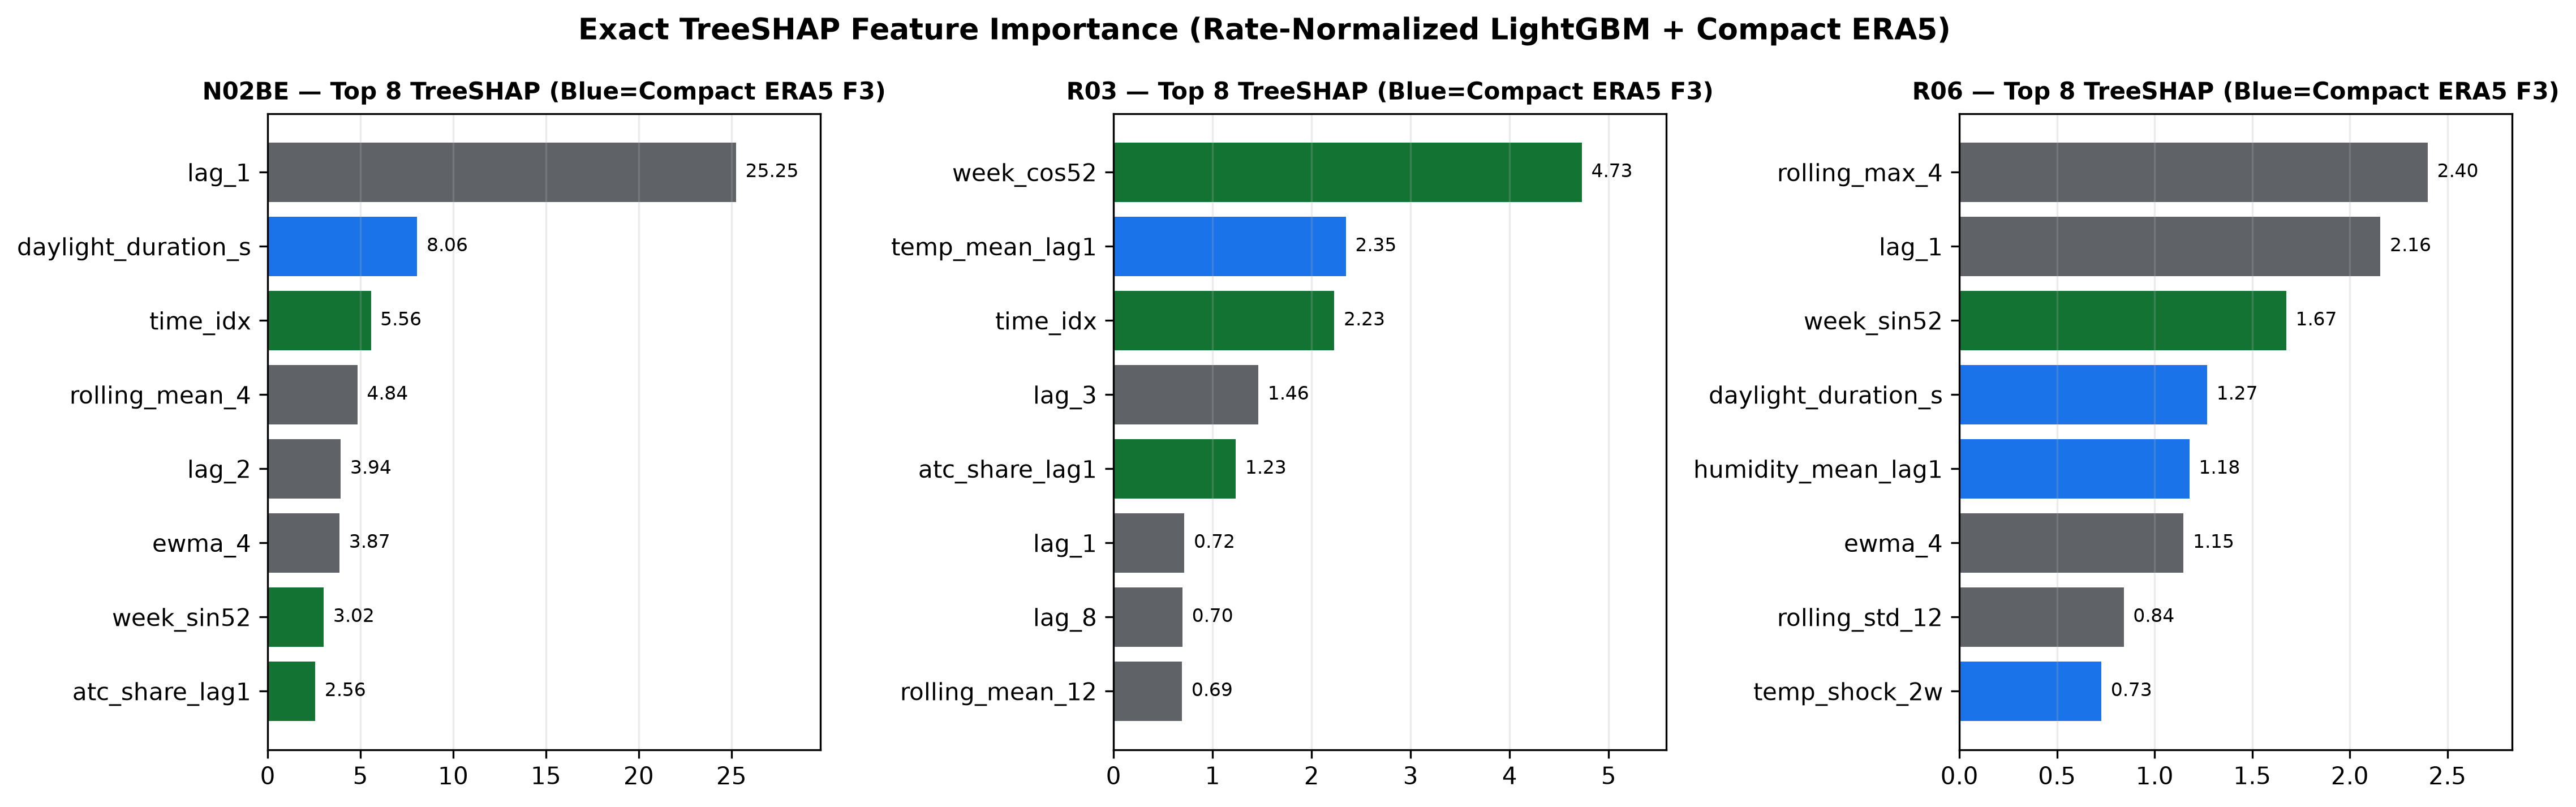
\includegraphics[width=\textwidth]{../../artifacts/forecasting/eval_treeshap_summary.png}
  \caption{Tỷ trọng giải thích \texttt{TreeSHAP} (\texttt{F1 / F2 / ERA5})}
  \label{fig:eval_shap}
\end{subfigure}
\caption{Kết quả bóc tách đặc trưng và giải thích TreeSHAP chứng minh đóng góp thời tiết ERA5}
\label{fig:eval_ablation_shap}
\end{figure}

\section{Thảo luận Trung thực Sai số và Giới hạn Quy mô Dữ liệu}
\begin{itemize}[leftmargin=1.5em]
  \item \textbf{Hai nhóm còn sau XGBoost của Paper 2024 (\texttt{M01AE} và \texttt{R03}):} Do nhóm khóa chặt quy tắc chọn mô hình theo Validation MAE (không nhìn tập Test) và giới hạn độ sâu cây để tránh quá khớp. Trên \texttt{4 Rolling Folds}, \texttt{Ridge} ổn định ở \texttt{M01AE} (\texttt{24.38 $\pm$ 6.83\%} WAPE) và \texttt{Croston\_SBA} đạt \texttt{37.58 $\pm$ 4.62\%} ở \texttt{R03}.
  \item \textbf{Nhóm bán thưa \texttt{N05C}:} Dù \texttt{Croston\_SBA} vượt MSE của \texttt{XGBoost} và \texttt{SNaïve\_W} trong \cite{fourkiotis2024}, WAPE vẫn ở mức \texttt{44.24--47.94\%} vì mẫu số trung bình tuần nhỏ (\texttt{4.14} đơn vị/tuần), nên khoảng tin cậy Split CQR (\texttt{86.5\%} độ phủ) đóng vai trò quyết định.
  \item \textbf{Giới hạn quy mô dữ liệu:} Theo nguyên tắc liêm chính của đề tài, bộ dữ liệu thực nghiệm hiện tại (\texttt{$\sim$715K} dòng POS và \texttt{19,902} tệp JSON thời tiết) đại diện cho quy mô \textit{chuỗi cửa hàng bán lẻ vừa}, chưa tự nhận là ``Big Data quy mô lớn'' dù kiến trúc S3 + Databricks Lakehouse đã sẵn sàng mở rộng theo chiều ngang khi tích hợp thêm dữ liệu POS nhiều năm.
\end{itemize}
